\documentclass[10pt, xcolor=dvipsnames]{beamer}
%\documentclass[10pt, xcolor=dvipsnames,notes=only]{beamer}
%\mode<presentation>
%{
\usetheme{Goettingen}
%\setbeamercovered{transparent}
%} 
\usefonttheme{professionalfonts}
%\usecolortheme{beaver}

\usepackage{setspace}
\usepackage[english]{babel}
\usepackage[latin1]{inputenc}
\usepackage{times}
\usepackage[T1]{fontenc}
\usepackage{color}
\usepackage{graphicx}
\usepackage{amssymb}
\usepackage{amsthm}
\usepackage{bm}
\usepackage{rotating}
\usepackage{ccaption}
\usepackage{booktabs}
\usepackage{lscape}
\usepackage{colortbl}
\usepackage{arydshln}
\usepackage{tabularx}
\usepackage{graphics}
\usepackage{epstopdf}

\setbeamertemplate{navigation symbols}{}
\setbeamertemplate{items}[balls]

\newenvironment{changemargin}[2]{%
  \begin{list}{}{%
    \setlength{\topsep}{0pt}%
    \setlength{\leftmargin}{#1}%
    \setlength{\rightmargin}{#2}%
    \setlength{\listparindent}{\parindent}%
    \setlength{\itemindent}{\parindent}%
    \setlength{\parsep}{\parskip}%
  }%
  \item[]}{\end{list}}

\setbeamercolor{block title}{fg=white, bg=teal}
\setbeamercolor{block body}{bg=teal!25}

\author[]{Chad Jones and Dietrich Vollrath}
\institute[Intro Growth]{Introduction to Economic Growth}
\date[]{}


\title[Endogenous Growth]{Evaluating Endogenous Growth Models}

\begin{document}
\maketitle

\section{Romer versus Schumpteter}
\begin{frame}{How they are the same}
The Romer and Schumpeter models share a lot of features:
\begin{itemize}
	\item The long-run growth rate is $g_A = g_L \lambda/(1-\phi)$
	\item The allocation $s_R$ does not influence the long-run growth rate
	\item Capital accumulation operates just like the Solow model
	\item The motive for innovation is capturing profits via monopolies
\end{itemize}
\end{frame}

\begin{frame}{How they are different}
The Romer and Schumpeter models have distinctions:
\begin{itemize}
	\item The notion of technology is different: new products (Romer) versus better products (Schumpeter)
	\item Firms persist in Romer, they are replaced in Schumpeterian model
	\item Additional factor in $s_R$ for Schumpeter, the probability of replacement
	\item If $g_A < r - g_L$, then $s_R$ is higher in Schumpeter: discount rate on future is ``big''
	\item If $g_A > r - g_L$, then $s_R$ is higher in Romer: discount rate on future is ``small''
\end{itemize}
\end{frame}

\begin{frame}{What kind of innovation occurs?}
Both kinds of innovation obviously happen:
\begin{itemize}
	\item Klenow and Li (2020) estimate the importance of both
	\item 27\% of growth via new varieties (Romer)
	\item 13\% of growth via replacement by better versions (Schumpeter)
	\item The other 60\% is via ``own innovation'': existing firms improving own products
	\item Our models don't allow for this. Why?
\end{itemize}
\end{frame}

\begin{frame}{Own innovation}
Why didn't we have ``own innovation'' in our models?
\begin{itemize}
	\item Arrow replacement effect (Arrow, 1962). Existing firms destroy own profits by replacing varieties.
	\item Assumption of ``drastic'' innovation: older varieties assumed to be unprofitable
\end{itemize}
Can we think harder about this?
\begin{itemize}
	\item The Arrow effect is present no matter what.
	\item But innovation isn't always drastic,
	\item Which means firms may persist and want to innovate to ``take the lead'' again
	\item Which leads to complicated strategic considerations as they compete
\end{itemize}
\end{frame}

\section{Competition and Innovation}
\begin{frame}{Strategic considerations}
More nuance about how firms make choices. Will compare fixed cost of innovation to the \textit{change} in firm value from innovation,
\begin{equation}
	F = V_{new} - V_{old}.
\end{equation}
Our basic Schumpeterian and Romer models assumed $V_{old}$ was zero. 
\vspace{.25in}\noindent
The comparison of $V_{new}$ and $V_{old}$ depends on the level of competition between firms

\end{frame}

\begin{frame}{Competitive market}
Assume firms are ``close'' in product quality, and they are in a competitive market. Their products are close substitutes (e.g. gas) or easy to make close copies of (e.g. clothes). 
\begin{itemize}
	\item The value $V_{old} \approx 0$ because of the competition
	\item If they do innovation, $V_{new}$ would be very big, they ``escape competition''
	\item The gap is big and the incentive to innovate is high for \textit{both} firms
\end{itemize}
\end{frame}

\begin{frame}{Competitive market}
Assume firms are ``far'' in product quality, and there is a clear leader and follower. But this is still acompetitive market. 
\begin{itemize}
	\item The leader already has profits, so $V_{new} - V_{old} \approx 0$ (the Arrow effect)
	\item The follower can catch up, but that just makes them competitive, so $V_{new} - V_{old} \approx 0$. 
	\item Neither has a big incentive to innovate
\end{itemize}
\end{frame}

\begin{frame}{Competitive market}
In competitive markets:
\begin{itemize}
	\item Lots of innovation when neck-and-neck
	\item Which means there is quickly a leader and a follower
	\item At which point innovation slows down
	\item So the industry tends to end up with a leader and follower
	\item And little innovation overall
	\item And \textit{more} competition would \textit{not} make this better
\end{itemize}
\end{frame}

\begin{frame}{Non-competitive markets}
Assume firms are ``close'' in product quality, but they are in a non-competitive market. Think of firms that collude or have distinct segmented markets (e.g. hospitals or airlines)
\begin{itemize}
	\item They already earn profits, so $V_{old}$ is big. 
	\item The gain from innovation, $V_{new} - V_{old} \approx 0$
	\item Neither firm has an incentive to innovate. They can just keep their existing profits.
\end{itemize}
\end{frame}

\begin{frame}{Non-competitive markets}
Assume there is a clear leader and follower, but they are still in a non-competitive market.
\begin{itemize}
	\item The leader already has $V_{old}$ that is big. There is little gain to innovation
	\item The follower can innovate and split profits with the leader, $V_{new} - V_{old}$ is big
	\item Followers have a lot of incentive to innovate
\end{itemize}
\end{frame}

\begin{frame}{Non-competitive market}
In non-competitive markets:
\begin{itemize}
	\item Lots of innovation when there is a leader and follower
	\item Which means they are quickly even or equal
	\item At which point innovation slows down
	\item So the industry tends to end up with equal firms close in quality
	\item And little innovation overall
	\item And \textit{more} competition \textit{would} make this better
\end{itemize}
\end{frame}

\begin{frame}{More competition and innovation}
Comparing these situations gives us no clear answer on competition and innovation
\begin{itemize}
	\item When markets are competitive, more competition can lower innovation
	\item When markets are very uncompetitive, more competitive can raise innovation
	\item There is some middle ground of competition which maximizes innovation
	\item Firms need to fear being replaced
	\item But need to know they can hang onto some profits
	\item Perfect competition doesn't maximize growth
\end{itemize}
\end{frame}

\section{Business Dynamism}

\begin{frame}{Schumpeterian dynamics}
The Schumpeterian model explicitly links firm entry and exit and economic growth
\begin{itemize}
	\item We know the long-run growth rate doesn't depend on how fast firms turn over
	\item ..but the \textit{level} of productivity depends on $E[dN]$
	\item ..which influences how fast firms replace one another
\end{itemize}
\end{frame}

\begin{frame}{Declining rates of entry and exit}
\begin{center}
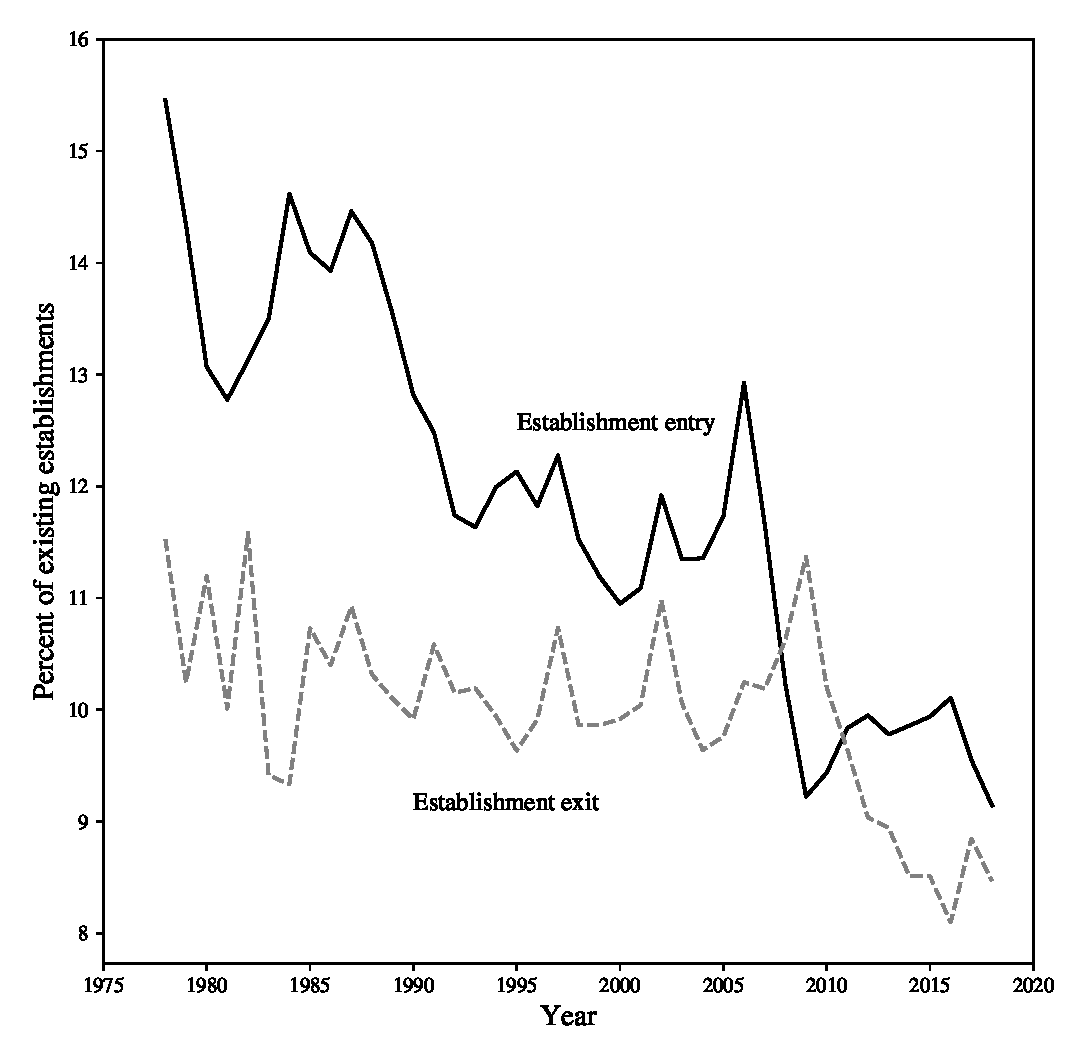
\includegraphics[height=3in]{../Figures/fig-ch6-fig2.eps}
\end{center}
\end{frame}

\begin{frame}{Implications}
If firm entry/exit is lower, this tracks to lower $E[dN]$ in the model:
\begin{itemize}
	\item Which could be indicative of lower $s_R$
	\item ..but measured $s_R$ appears higher (see Chapter 4)
	\item ..so either the measure of $s_R$ is imperfect (possible)
	\item ..OR something else changed in the economy
\end{itemize}
\end{frame}

\begin{frame}{Implications}
Assume $s_R$ did go up, but $E[dN]$ did fall, how might that work?
\begin{equation}
	\frac{s_R}{1-s_R} = \frac{\alpha(1-\alpha)}{(1-\alpha)}\frac{E[dN]}{r-g_A-g_L+E[dN]}. \nonumber
\end{equation}
One possibility is that $\alpha$ changed
\begin{itemize}
	\item If $\alpha(1-\alpha)$ goes up, the profit share goes up
	\item While $(1-\alpha0$ goes down, and the labor share falls
	\item This would drive firms to raise $s_R$
	\item And could offset a drop in $E[dN]$
\end{itemize}
Indicative of rise in ``winner-take-all'' innovation? 
\end{frame}

\section{Optimal R\&D}
\begin{frame}{Are we doing enough R\&D?}
There are several reasons $s_R$ won't be the optimal value. A first is:
\begin{itemize}
	\item Firms value profits of innovation, but do not take into account the effect of their innovation on others. 
	\item If $\phi<0$ raising $A$ lowers the innovation rate. Firms could do too \textit{much} innovation.
	\item Or if $\phi>0$ raising $A$ raises the innovation rate. Firms do too \textit{little} innovation.
\end{itemize}

\end{frame}

\begin{frame}{Are we doing enough R\&D?}
A second reason $s_R$ isn't optimal:
\begin{itemize}
	\item If $\lambda < 1$, then doing R\&D crowds others, lowering the rate of innovation
	\item In this sense firms do too \textit{much} innovation
	\item R\&D would be improved if more coordinated
\end{itemize}

\end{frame}

\begin{frame}{Are we doing enough R\&D?}
A third reason $s_R$ isn't optimal:
\begin{itemize}
	\item To ensure economic profits we need to make ideas excludable
	\item That happens via patents, copyrights, etc.
	\item These rights give firms monopolies, or market power, over that idea
	\item Monpolists tend to under-produce while maximizing profits
	\item Consumers would like it if innovators produced more at a lower price
	\item There is too \textit{little} innovation because firms only account for their profits
\end{itemize}

\end{frame}

\begin{frame}{The social return to R\&D}
Jones and Summers (2020) try to calculate the social value of R\&D. The PDV of GDP per capita given growth of $g_A$ is
\begin{equation}
	\frac{y_0}{r-g_A}
\end{equation}
givn initial value of $y_0$ and a discount rate of $r$. If there was \textit{no} innovation, the PDV would be
\begin{equation}
	\frac{y_0}{r}
\end{equation}
so the benefit of R\&D is
\begin{equation}
	\text{Benefits} = y_0\left(\frac{1}{r-g_A} - \frac{1}{r}\right).
\end{equation}
\end{frame}

\begin{frame}{The costs of R\&D}
The costs of R\&D are the resources and workers we apply to R\&D, who don't produce goods and services in the near term. 
\begin{equation}
	\text{Costs} = \frac{w_0s_R}{r-g_A}. \nonumber
\end{equation}
where $w_0 s_R$ are the wages of the fraction $s_R$ of all workers who do R\&D. 
\end{frame}

\begin{frame}{Benefit/Cost ratio}
Calculate the ratio of benefits to costs as:
\begin{eqnarray}
	\rho &=& \frac{\text{Benefits}}{\text{Costs}} \nonumber  \\ 
	     &=& \frac{y_0\left(\frac{1}{r-g_A} - \frac{1}{r}\right)}{\frac{w_0}{r-g_A}} \nonumber \\ 
	     &=& \frac{y_0}{w_0s_R}\frac{g_A}{r} \nonumber \\ 
	     &=& \frac{g_A/r}{(1-\alpha)s_R} \nonumber
\end{eqnarray}
Benefits are high if $g_A$ is high and/or $s_R$ is low. 
\end{frame}

\begin{frame}{Quantifying the benefits}
Let $g_A = 0.018$, $r=0.05$, $(1-\alpha)s_R = 0.027$, meaning R\&D costs 2.7\% of GDP.
\begin{equation}
	\rho \approx \frac{0.018/0.05}{0.027} = 13.3. \nonumber
\end{equation}
One dollar of R\&D returns about 13 dollars of present value. A huge return! Implication is that we should do a \textit{lot} more R\&D. Jones/Summers calculate that if R\&D cost around 50\% of GDP, it would still be worth it!
\end{frame}

\begin{frame}{Why is R\&D so powerful?}
What makes R\&D and innovation so valuable?
\begin{itemize}
	\item R\&D uses rival inputs (workers, some capital) \textit{today}
	\item But produces non-rival ideas that can be used by others
	\item And can be used \textit{forever} (or at least a long time)
\end{itemize}
\end{frame}

\end{document}